% dit commando is nodig om 2 plaatjes in 1 tabel te duwen
\newcommand{\cegraphic}[2]{{\renewcommand{\arraystretch}{0}
			    \begin{tabular}{c}%
			     \vrule height 0pt width 0pt\\
			     \includegraphics[#1]{#2}\\
			     \vrule height 0pt width 0pt
			    \end{tabular}}}

\section[Achtergrond]{Achtergrondinformatie}
\label{achtergrondinfo}

\subsection{De pers}

Om een goede indruk van een \index{Drukpers}drukpers te krijgen, zijn hieronder wat plaatjes te zien van een pers met daarin een metalen plaat die gebogen wordt:

\begin{figure}[h]
\begin{tabular}{cc}
\cegraphic{height=5cm}{pers1.jpg}&
\cegraphic{height=5cm}{pers2.jpg}
\end{tabular}
\end{figure}

Zoals in de plaatjes boven te zien is, wordt een product\footnote{In de plaatjes de blauwe plaat} gebogen doordat de \index{Persbalk}\emph{persbalk} naar beneden beweegt. Hierdoor komt de \index{Stempel}\emph{stempel} tegen het product aan, die door de \index{Matrijs}\emph{matrijs} tegengehouden wordt. De plaat hiertussen verbuigt daardoor, hetgeen resulteert in een buiging. De \index{Vingers}\emph{vingers} ondersteunen hierbij het product, zodat het op zijn plaats blijft.

\subsection{De modules}
\label{module}
De persbalk en de vingers worden aangestuurd door zogenaamde \index{Module}modules, die via een CAN\footnote{Controller Area Network, Ook wel bekend als HSB-bus} door de \index{Besturing}besturing\footnote{Op de vorige pagina het kastje uiterst links} worden aangestuurd.

Een overzicht van de besturing met de modules:

\begin{figure}[h]
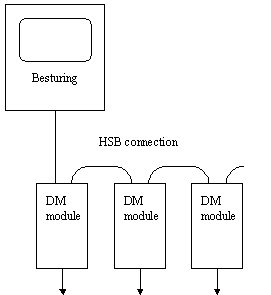
\includegraphics[width=6.5cm]{hsb.jpg}
\end{figure}

Deze stageopdracht richt zich op de DM modules, en niet op de besturing zelf. De modules zelf sturen bijvoorbeeld motoren aan, of staan in verbinding met sensoren.
